\باب{برقرار مقناطیسی میدان}
برقی میدان کا منبع برقی چارج ہے جس پر باب \حوالہ{باب_کولومب_قانون} میں تفصیلی غور کیا گیا۔مقناطیسی میدان کا منبع یا تو مقناطیس ہو سکتا ہے، یا وقت کے ساتھ بدلتا برقی میدان اور یا پھر برقی رو۔اس کتاب میں مقناطیس سے پیدا مقناطیسی میدان پر غور نہیں کیا جائے گا۔وقت کے ساتھ بدلتے برقی میدان سے پیدا مقناطیسی میدان پر ایک اور باب میں غور کیا جائے گا جبکہ اس باب میں برقی رو سے پیدا مقناطیسی میدان پر غور کیا جائے گا۔

\حصہ{بایوٹ-سیوارٹ کا قانون}
برقی رو اور اس سے پیدا مقناطیسی میدان کا تعلق \اصطلاح{بایوٹ-سیوارٹ}\فرہنگ{بایوٹ-سیوارٹ}\حاشیہب{Biot-Savart law}\فرہنگ{Biot-Savart law} کا قانون\حاشیہد{یہ قانون فرانس کے  بایوٹ اور سیوارٹ نے 1820 میں پیش کیا۔یہ دونوں ایمپیئر کے ساتھی تھے۔}
\begin{align}\label{مساوات_بایوٹ_سیوارٹ_تفرق_شکل}
\dif \kvec{H}=\frac{I \dif \kvec{L} \times \aR}{4 \pi R^2}
\end{align}
 بیان کرتا ہے جہاں سے مقناطیسی شدت \عددیء{\kvec{H}} کی اکائی ایمپیئر فی میٹر \عددیء{(\si{\ampere \per \meter})} حاصل ہوتی ہے۔آئیں اس قانون کا مطلب سمجھیں۔

یہ قانون باریک تار کے انتہائی چھوٹے حصے \عددیء{\dif \kvec{L}} جس میں \عددیء{I} برقی رو گزر رہا ہو سے  نقطہ \عددیء{P} پر پیدا سمتی برقی میدان \عددیء{\kvec{H}} دیتا ہے۔نقطہ \عددیء{P} باریک تار کے چھوٹی لمبائی سے \عددیء{\kvec{R}} فاصلے پر ہے۔باریک تار سے مراد ایسی ٹھوس نلکی نما موصل تار ہے جس کے رقبہ عمودی تراش کا رداس اتنا کم کر دیا جائے کہ یہ صفر کے قریب تر ہو۔\عددیء{\dif \kvec{L}} کی سمت برقی رو کی سمت میں ہے جبکہ \عددیء{I \dif \kvec{L}} منبع مقناطیسی میدان ہے۔

مقناطیسی شدت کی قیمت برقی رو ضرب باریک چھوٹی تار کی لمبائی ضرب \عددیء{\kvec{R}} اور \عددیء{\dif \kvec{L}} کے مابین زاویہ کے سائن کے برائے راست تناسب جبکہ ان کے مابین فاصلہ \عددیء{R} کے مربع کے بالعکس تناسب رکھتی ہے۔تناسبی مستقل \عددیء{\tfrac{1}{4\pi}} ہے۔

بایوٹ-سیوارٹ کے  قانون کا موازنہ کولومب کے قانون کے ساتھ کرنے کی غرض سے دونوں مساوات کو ایک ساتھ لکھتے ہیں۔
\begin{align*}
\dif \kvec{H}_2&=\frac{I_1 \dif \kvec{L}_1 \times \kvec{a}_{R21}}{4 \pi R_{21}^2}\\
\dif \kvec{E}_2&=\frac{\dif Q_1 \kvec{a}_{R21}}{4\pi \epsilon_0 R_{21}^2}
\end{align*}
ان مساوات میں زیر نوشت میں \عددیء{2} اس مقام کو ظاہر کرتی ہے جہاں میدان کی قیمت حاصل کی گئی ہے جبکہ زیر نوشت میں \عددیء{1} میدان کے منبع کے مقام کو ظاہر کرتی ہے۔دونوں میدان فاصلے کے مربع کا بالعکس تناسب رکھتے ہیں۔دونوں اقسام کے میدان کی شدت اور میدان کی منبع کا خطی تعلق ہے۔دونوں میں فرق میدان کی سمت کا ہے۔برقی میدان کی سمت منبع سے اس نقطہ کی جانب ہے جہاں میدان حاصل کیا جا رہے ہو۔مقناطیسی میدان کی سمت سمتی ضرب کے دائیں ہاتھ کے قانون سے حاصل ہوتی ہے۔

بایوٹ-سیوارٹ کے قانون کو مساوات \حوالہ{مساوات_بایوٹ_سیوارٹ_تفرق_شکل} کی شکل میں تجرباتی طور پر ثابت نہیں کیا جا سکتا چونکہ باریک تار کے چھوٹی لمبائی میں برقی رو تب گزرے گی جب یہ اس تک پہنچائی جائے۔جو تار اس تک برقی رو پہنچائے گا، وہ بھی مقناطیسی میدان پیدا کرے گا۔انہیں علیحدہ علیحدہ نہیں کیا جا سکتا۔یوں بایوٹ-سیوارٹ قانون کی تکمل شکل
\begin{align}\label{مساوات_بایوٹ_سیوارٹ_تکمل_شکل}
\kvec{H}=\oint \frac{I \dif \kvec{L} \times \aR}{4 \pi R^2}
\end{align}
ہی تجرباتی طور ثابت کی جا سکتی ہے۔

مساوات \حوالہ{مساوات_بایوٹ_سیوارٹ_تفرق_شکل} سے مساوات \حوالہ{مساوات_بایوٹ_سیوارٹ_تکمل_شکل} لکھی جا سکتی ہے۔البتہ مساوات \حوالہ{مساوات_بایوٹ_سیوارٹ_تکمل_شکل} میں تکمل کے اندر کوئی بھی ایسی اضافی تفاعل شامل کیا جا سکتا ہے جس کا بند تکمل صفر کے برابر ہو۔مقداری میدان کا ڈھلان ہر صورت بقائی میدان ہوتا ہے لہٰذا مساوات \حوالہ{مساوات_بایوٹ_سیوارٹ_تکمل_شکل} میں \عددیء{\nabla G} کے شمول سے اس کے جواب میں کوئی فرق نہیں پڑے گا۔\عددیء{G} کوئی بھی مقداری میدان ہو سکتا ہے۔اس حقیقت کا تذکرہ اس لئے کیا جا رہا ہے کہ اگر ہم ایک چھوٹے برقی رو گزارتے تار پر دوسرے  چھوٹے برقی رو گزارتے تار سے پیدا قوت دریافت کرنا چاہیں جہاں تجرباتی طور پر ان کا میدان قابل دریافت نہ ہو تب ہمیں احمقانہ جوابات ہی حاصل ہوں گے۔

بایوٹ-سیوارٹ کے قانون کو سطحی کثافت برقی رو \عددیء{\kvec{K}} یا کثافت برقی رو \عددیء{\kvec{J}} کی صورت میں بھی لکھا جا سکتا ہے جہاں
\begin{align}
I \dif \kvec{L}=\kvec{K} \dif S=\kvec{J} \dif v
\end{align}
لکھا جائے گا۔ یوں بایوٹ-سیوارٹ کے قانون کو
\begin{align}
\kvec{H}=\int_S \frac{\kvec{K} \times \aR \dif S}{4\pi R^2}
\end{align}
یا
\begin{align}
\kvec{H}=\int_h \frac{\kvec{J} \times \aR \dif h}{4\pi R^2}
\end{align}
لکھا جا سکتا ہے۔

\begin{figure}
\centering
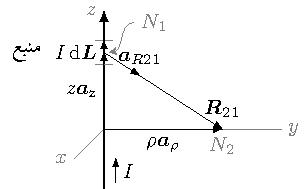
\includegraphics{figMagneticInfiniteStraightWiresField}
\caption{سیدھی لامحدود تار سے پیدا مقناطیسی میدان}
\label{شکل_مقناطیسی_سیدھی_لامحدود_تار_کا_میدان}
\end{figure}
آئیں برقی رو گزارتے سیدھی  لامحدود لمبائی کے تار سے پیدا مقناطیسی میدان بایوٹ-سیوارٹ کے قانون سے حاصل کریں۔شکل \حوالہ{شکل_مقناطیسی_سیدھی_لامحدود_تار_کا_میدان} میں صورت حال دکھائی گئی ہے۔اس تار کے دونوں سرے لامحدود فاصلے پر ہیں۔تار کے قریب نقطہ \عددیء{N} پر مقناطیسی میدان کا بیشتر حصہ تار کے اس حصے کی وجہ سے ہو گا جو \عددیء{N} کے قریب ہو۔یوں لامحدود فاصلے پر تار کے سروں تک برقی رو پہنچانے  والے تار کا نقطہ \عددیء{N} پر اثر کو نظرانداز کرتے ہوئے آگے بڑھتے ہیں۔ 

نقطہ \عددیء{N_1} پر تار کے چھوٹے حصے \عددیء{\dif \kvec{L}} کو منبع مقناطیسی میدان تصور کرتے ہوئے مساوات \حوالہ{مساوات_بایوٹ_سیوارٹ_تفرق_شکل} کی مدد سے نقطہ \عددیء{N_2} پر مقناطیسی میدان لکھی جا سکتی ہے۔چونکہ 
\begin{align*}
\kvec{R}_{21}=\rho \arho-z \az
\end{align*}
کے برابر ہے لہٰذا
\begin{align*}
R_{21}&=\abs{\kvec{R}_{21}}=\sqrt{\rho^2+z^2}\\
\aR&=\frac{\kvec{R}_{21}}{\abs{\kvec{R}_{21}}}=\frac{\rho \arho-z \az}{\sqrt{\rho^2+z^2}}
\end{align*}
لکھے جا سکتے ہیں۔نلکی محدد میں چھوٹی لمبائی
\begin{align*}
\dif \kvec{L}=\dif \rho \arho+\rho \dif \phi \aphi+\dif z \az
\end{align*}
لکھی جاتی ہے۔چونکہ یہاں \عددیء{\dif \rho=0} اور \عددیء{\dif \phi=0} ہیں لہٰذا \عددیء{\dif \kvec{L}=\dif z \az} لکھتے ہوئے  مساوات \حوالہ{مساوات_بایوٹ_سیوارٹ_تفرق_شکل} کو
\begin{align*}
\dif \kvec{H}_2=\frac{I \dif z \az \times (\rho \arho -z\az)}{4 \pi (\rho^2+z^2)^{\frac{3}{2}}}
\end{align*}
لکھا جا سکتا ہے۔پورے تار کا مقناطیسی میدان اس مساوات کے تکمل سے حاصل ہو گا جہاں تکمل\عددیء{-\infty} تا \عددیء{+\infty} حاصل کیا جائے گا۔اس طرح
\begin{align*}
\kvec{H}_2&=\int_{-\infty}^{\infty}\frac{I \dif z \az \times (\rho \arho -z\az)}{4 \pi (\rho^2+z^2)^{\frac{3}{2}}}\\
&=\frac{I \rho}{4\pi}\int_{-\infty}^{\infty} \frac{\aphi \dif z }{(\rho^2+z^2)^{\frac{3}{2}}}
\end{align*}    
لکھا جا سکتا ہے جہاں صفحہ \حوالہصفحہ{مساوات_سمتیات_نلکی_اکائی_سمتیات_کا_سمتی_ضرب} پر مساوات \حوالہ{مساوات_سمتیات_نلکی_اکائی_سمتیات_کا_سمتی_ضرب} کی مدد سے \عددیء{\az \times \arho=\aphi} جبکہ مساوات \حوالہ{مساوات_سمتیات_نلکی_اکائی_سمتیات_کا_سمتی_ضرب_ب} کی مدد سے \عددیء{\az \times \az=0} لکھے گئے ہیں۔

مندرجہ بالا مساوات میں تکمل کے اندر \عددیء{\aphi} پر نظر رکھنا ہو گا۔اگرچہ \عددیء{\aphi} اکائی سمتیہ ہے لہٰذا اس کی لمبائی تبدیل نہیں ہو سکتی البتہ یہ دیکھنا ضروری ہے کہ آیا تکمل کا متغیرہ یعنی \عددیء{z} تبدیل کرنے سے \عددیء{\aphi} کی سمت تو تبدیل نہیں ہوتی۔صفحہ \حوالہصفحہ{مساوات_سمتیہ_اکائی_زاویہ_کارتیسی_میں} پر مساوات \حوالہ{مساوات_سمتیہ_اکائی_زاویہ_کارتیسی_میں} کے تحت
\begin{align*}
\aphi&=-\frac{y}{\sqrt{x^2+y^2}} \ax+\frac{x}{\sqrt{x^2+y^2}} \ay
\end{align*}
لکھا جا سکتا ہے۔آپ دیکھ سکتے ہیں کہ \عددیء{z} تبدیل کرنے سے \عددیء{\aphi} پر کوئی اثر نہیں پڑتا لہٰذا \عددیء{\aphi} کو تکمل کے باہر منتقل کیا جا سکتا ہے۔یوں
\begin{gather}
\begin{aligned}\label{مساوات_مقناطیسی_سیدھی_لامحدود_تار_کا_میدان}
\kvec{H}_2&=\frac{I \rho\aphi}{4\pi}\int_{-\infty}^{\infty} \frac{\dif z }{(\rho^2+z^2)^{\frac{3}{2}}}\\
&=\eval{\frac{I \rho \aphi}{4\pi} \frac{z}{\rho^2 \sqrt{\rho^2+z^2}}}_{-\infty}^{+\infty}
\end{aligned}
\end{gather}    
سے
\begin{align}
\kvec{H}_2=\frac{I}{2\pi \rho} \aphi
\end{align}
حاصل ہوتا ہے۔شکل \حوالہ{شکل_مقناطیسی_سیدھے_تار_کا_میدان_دائرے} میں برقی رو صفحہ سے باہر نکل رہی ہے جبکہ گول دائرے مقناطیسی میدان کو ظاہر کرتے ہیں۔اگر تار کو دائیں ہاتھ سے یوں پکڑا جائے کہ انگوٹھا برقی رو کی سمت میں ہو تب اس ہاتھ کی انگلیاں تار کے گرد مقناطیسی میدان کی سمت میں لپٹی ہوں گی۔آپ دیکھ سکتے ہیں کہ یہ مقناطیسی میدان نا نو \عددیء{z} اور نا ہی زاویہ \عددیء{\phi} کے ساتھ تبدیل ہوتا ہے۔اس کی قیمت صرف تار سے فاصلے پر منحصر ہے۔
\begin{figure}
\centering
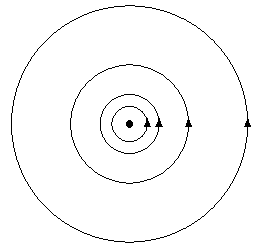
\includegraphics{figMagneticInfiniteStraightWiresStreamlines}
\caption{سیدھی لمبی تار کا مقناطیسی میدان تار کے گرد دائرے بناتا ہے۔برقی رو صفحے سے باہر نکل رہی ہے۔}
\label{شکل_مقناطیسی_سیدھے_تار_کا_میدان_دائرے}
\end{figure}
%
\begin{figure}
\centering
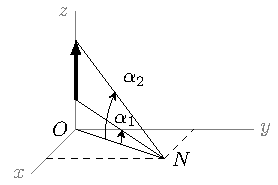
\includegraphics{figMagneticStraightWiresField}
\caption{سیدھی  محدود لمبائی کے تار کی مقناطیسی شدت۔}
\label{شکل_مقناطیسی_سیدھے_محدود_تار_کا_میدان}
\end{figure}

اگر شکل \حوالہ{شکل_مقناطیسی_سیدھی_لامحدود_تار_کا_میدان} میں تار لامحدود نہ ہو تب مساوات \حوالہ{شکل_مقناطیسی_سیدھے_محدود_تار_کا_میدان} میں تکمل کے محدود حدود پر کرنے سے مقناطیسی میدان کی شدت
\begin{align}\label{مساوات_مقناطیسی_محدود_تار_کی_مقناطیس}
\kvec{H}=\frac{I}{4\pi \rho} \left(\sin \alpha_2-\sin \alpha_1 \right) \aphi
\end{align}
حاصل ہوتی ہے جہاں شکل \حوالہ{شکل_مقناطیسی_سیدھے_محدود_تار_کا_میدان} میں \عددیء{\alpha_1} اور \عددیء{\alpha_2} کی نشاندہی کی گئی ہے۔تار کا نچلا سرا \عددیء{xy} سطح یعنی \عددیء{z=0} سطح سے نیچے ہونے کی صورت میں \عددیء{\alpha_1} کی قیمت منفی ہو گی۔یہی کچھ تار کے دوسرے سرے اور \عددیء{\alpha_2} کے لئے بھی درست ہے۔

\حصہ{ایمپیئر کا دوری قانون}
کولومب کے قانون کی مدد سے مختلف طرز پر پائے جانے والے چارج کے برقی میدان حاصل کرنے کے بعد ہم نے گاؤس کا قانون اخذ کیا جس سے ہماری زندگی نہایت آسان ہو گئی۔گاؤس کے قانون کی مدد سے متشاکل چارج سے پیدا برقی میدان انتہائی آسانی سے حاصل ہوتا ہے۔متشاکل برقی رو کے مقناطیسی میدان حاصل کرنے کا بھی اتنا ہی آسان طریقہ موجود ہے جسے \اصطلاح{ایمپیئر کا دوری قانون}\فرہنگ{ایمپیئر کا دوری قانون}\حاشیہب{Ampere's circuital law}\فرہنگ{Ampere's circuital law} کہتے ہیں۔اس قانون کو بایوٹ-سیوارٹ کے قانون سے آگے جا کر حاصل کیا گیا ہے۔فی الحال ہم اس قانون کو استعمال کرنا سیکھتے ہیں۔اس قانون کے استعمال کے وقت مسئلے پر غور کرتے ہوئے بغیر حساب و کتاب کے فیصلہ کیا جاتا ہے کہ مقناطیسی میدان کے کون کون سے اجزاء موجود نہیں ہونے چاہئے۔یہ فیصلہ برقی رو کے راستے کو دیکھ کر کیا جاتا ہے۔

ایمپیئر کا دوری قانون کہتا ہے کہ یک سمتی برقی رو کے گرد کسی بھی راہ \عددیء{\kvec{H}} کا لکیری بند تکمل گھیرے برقی رو کے برابر ہو گا یعنی
\begin{align}\label{مساوات_مقناطیسی_ایمپیئر_کا_دوری_قانون}
\oint \kvec{H} \cdot \dif \kvec{L}=I
\end{align}

لکیری بند تکمل کی سمت میں برقی رو کے گرد  دائیں ہاتھ کی انگلیاں گھمانے سے اسی ہاتھ کا انگوٹھا مثبت برقی رو کی سمت دے گا۔ایسا کرتے وقت انگوٹھے کو باقی چار انگلیوں کے عمودی رکھا جاتا ہے۔

کسی بھی راہ \عددیء{\kvec{H}} کے لکیری تکمل سے مراد اس راہ  کو انتہائی چھوٹے چھوٹے ٹکڑوں \عددیء{\dif \kvec{L}} میں تقسیم کر کے ہر ٹکڑے پر \عددیء{\kvec{H}} کی قیمت استعمال کرتے ہوئے \عددی{\kvec{H} \cdot \dif \kvec{L}} حاصل کر کے تمام \عددی{\kvec{H} \cdot \dif \kvec{L}} کا مجموعہ حاصل کرنا ہے۔مقناطیسی شدت \عددیء{\kvec{H}} کی قیمت مختلف مقامات پر عموماً مختلف ہو گی۔یوں کسی ایک نقطے پر \عددی{\kvec{H} \cdot \dif \kvec{L}} کی قیمت کسی دوسرے نقطے کے \عددی{\kvec{H} \cdot \dif \kvec{L}} سے مختلف ہو گی۔ایمپیئر کا دوری قانون کہتا ہے کہ اگرچہ یک سمتی برقی رو کے گرد دو مختلف بند راہوں پر جگہ جگہ \عددی{\kvec{H} \cdot \dif \kvec{L}} کی قیمتیں مختلف ہوں گی لیکن دونوں راہ پر ان کا مجموعہ عین برقی رو کے برابر ہو گا۔

کسی بھی سطح کا محیط، بند راہ ہوتی ہے۔اسی طرح کوئی بھی بند راہ، لامحدود سطحوں کا محیط ہوتا ہے۔یوں بند راہ کا گھیرا ہوا برقی رو ان تمام سطحوں کو چھیرتا ہوا گزرے گا جن کا محیط یہ بند راہ ہو۔

گاؤس کے قانون کا استعمال تب ممکن ہوتا ہے جب بند سطح میں کل برقی چارج معلوم ہو۔ایمپیئر کا دوری قانون اس صورت استعمال کیا جا سکتا ہے جب  بند راہ میں گھیرا کل یک سمتی برقی رو معلوم ہو۔   

آئیں شکل \حوالہ{شکل_مقناطیسی_سیدھی_لامحدود_تار_کا_میدان} میں دکھائے گئے  برقی رو گزارتے سیدھی لامحدود لمبائی کے تار کی مقناطیسی شدت ایمپیئر کے دوری قانون یعنی مساوات \حوالہ{مساوات_مقناطیسی_ایمپیئر_کا_دوری_قانون} کی مدد سے دوبارہ حاصل کریں۔اس مساوات کو استعمال کرتے ہوئے  برقی رو کے گرد راہ یوں چنی جاتے ہے کہ اس پر \عددیء{\kvec{H}} اور \عددیء{\dif \kvec{L}} یا تو آپس میں عمودی ہوں اور یا \عددیء{\kvec{H}} کی قیمت قطعی اور اس کی سمت \عددیء{\dif \kvec{L}} کے متوازی ہو۔پہلی صورت میں دونوں متغیرات کے مابین نوے درجے کا زاویہ  ہے اور \عددیء{\cos 90\degree=0} ہوتا ہے لہٰذا \عددیء{\kvec{H} \cdot \dif \kvec{L}} صفر کے برابر ہو گا اور یوں راہ کے اس حصے پر تکمل صفر کے برابر ہو گا۔ دوسری صورت میں متغیرات کے مابین صفر درجے کا زاویہ ہے اور \عددیء{\cos 0 \degree=1} ہوتا ہے لہٰذا \عددیء{\kvec{H} \cdot \dif \kvec{L}}  کو \عددیء{H \dif L} لکھا جا سکتا ہے اور ساتھ ہی ساتھ مقناطیسی شدت کی قیمت قطعی ہونے کی وجہ سے \عددیء{H} کو تکمل کے باہر لے جایا جا سکتا ہے۔یوں راہ کے اس راستے پر تکمل کی قیمت \عددیء{H L} کے برابر ہو گی جہاں \عددیء{L} راہ کے اس حصے کی لمبائی ہے۔

تار کے گرد اور اس کے ساتھ ساتھ حرکت کرنے سے واضح ہوتا ہے کہ مسئلے کی نوعیت نا تو تار کے گرد زاویہ \عددیء{\phi} پر اور نا ہی محدد \عددیء{z} پر منحصر ہے۔تار سے دور یا اس کے قریب ہونے سے ہی مسئلے کی نوعیت میں تبدیلی آتی ہے۔یوں صاف ظاہر ہے کہ مقناطیسی شدت صرف \عددیء{\rho} پر منحصر ہو سکتی ہے۔اسی طرح بایوٹ-سیوارٹ کے قانون کو مد نظر رکھتے ہوئے ہم دیکھ سکتے ہیں کہ مقناطیسی شدت \عددیء{\aphi} سمت رکھتی ہے یعنی اس کا صرف \عددیء{H_{\phi}} جزو پایا جائے گا۔یوں اگر \عددیء{\rho} تبدیل کئے بغیر تار کے گرد چلا جائے تو ہم یقین رکھ سکتے ہیں کہ \عددیء{\kvec{H}} کی حتمی قیمت \عددیء{H_{\phi}} تبدیل نہیں ہو گی۔ساتھ ہی ساتھ اس راہ پر کسی بھی نقطے پر  \عددیء{\dif \kvec{L}=\rho \dif \phi \aphi} اور \عددیء{H_{\phi} \aphi} آپس میں متوازی ہوں گے لہٰذا ایمپیئر کے دوری قانون سے
\begin{align*}
\oint \kvec{H} \cdot \dif \kvec{L}=\int_0^{2\pi} H_{\phi} \rho \dif \phi=H_{\phi} \rho \int_0^{2\pi} \dif \phi=H_{\phi} 2\pi \rho=I
\end{align*}
یا
\begin{align*}
H_{\phi}=\frac{I}{2\pi \rho}
\end{align*}
حاصل ہوتا ہے جو ہم پہلے بھی حاصل کر چکے ہیں۔
\begin{figure}
\centering
\begin{subfigure}{0.5\textwidth}
\centering
\includegraphics{figGaussCoaxialThickOuterWallUnshaded}
\caption{ہم محوری تار کے اندرونی تار میں مثبت جبکہ بیرونی تار میں منفی برقی رو ہے۔}
\label{شکل_مقناطیسی_ہم_محوری_تار_مثبت_منفی_رو}
\end{subfigure}%
\begin{subfigure}{0.5\textwidth}
\centering
\includegraphics{figGaussCoaxialRadialComponentsCancelOut}
\caption{رداسی اجزاء آپس میں ختم ہو جاتے ہیں اور یوں صرف زاویاتی جزو رہ جاتا ہے۔}
\label{شکل_مقناطیسی_ہم_محوری_صرف_زاویاتی_جزو}
\end{subfigure}%
\caption{ہم محوری تار۔}
\label{شکل_مقناطیسی_ہم_محوری_تار}
\end{figure}

ایمپیئر کے دوری قانون  کے استعمال کی دوسری مثال کی خاطر ہم شکل \حوالہ{شکل_مقناطیسی_ہم_محوری_تار} میں دکھائے گئے ہم محوری تار لیتے ہیں۔فرض کریں کہ \عددیء{z} محدد پر پڑی  ایسی لامحدود لمبائی کے ہم محوری  تار کے اندرونی حصے میں \عددیء{I} اور اس کے بیرونی سطح میں \عددیء{-I} برقی رو گزر رہی ہے۔اندرونی موصل موٹی ساخت کے تار کو نہایت پتلی فرضی تاروں کا مجموعہ تصور کیا جا سکتا ہے۔آئیں ان پتلی فرضی تاروں سے نقطہ \عددیء{N} پر پیدا مقناطیسی شدت پر غور کریں۔نقطہ \عددیء{N} کو کارتیسی محدد کے \عددیء{x} محدد پر رکھتے ہوئے مسئلے کی نوعیت شکل \حوالہ{شکل_مقناطیسی_ہم_محوری_تار}-ب میں دکھائی گئی ہے۔پچھلی مثال سے یہ واضح ہے کہ ایسی کسی بھی پتلی تار کی مقناطیسی شدت میں \عددیء{H_z} جزو نہیں پایا جاتا۔ساتھ ہی ساتھ ہم یہ بھی جانتے ہیں کہ ایسی تار کی مقناطیسی شدت تار کے گرد گول دائرہ بناتی ہے۔کسی بھی فرضی تار جو \عددیء{(\rho_0,\phi_0)} پر پایا جاتا ہو \عددیء{N} پر  \عددیء{\Delta H_{\rho}} اور \عددیء{\Delta H_{\phi}} اجزاء پیدا کرے گا۔اسی طرح \عددیء{(\rho_0,-\phi_0)} پر پتلی تار سے پیدا مقناطیسی شدت کے بھی ایسے رداسی اور زاویاتی اجزاء ہوں گے۔ان دونوں پتلی تاروں کے رداسی اجزاء آپس میں الٹ سمت میں ہوں گے لہٰذا یہ ایک دونوں کو ختم کرتے ہیں جبکہ زاویاتی اجزاء ایک ہی سمت میں ہوتے ہیں لہٰذا \عددیء{N} پر صرف زاویاتی جزو پایا جائے گا۔

اندرونی ٹھوس موصل تار کے گرد ایسا گول دائرہ لیتے ہیں جس کا رداس \عددیء{\rho} اندرونی تار کے رداس \عددیء{\rho_1} سے زیادہ مگر بیرونی تار کے اندرونی رداس \عددیء{\rho_2} سے کم ہو۔اس راہ پر ہم ایمپیئر کے دوری قانون کی مدد سے
\begin{align*}
H_{\phi}=\frac{I}{2\pi \rho} \quad \quad (\rho_1 < \rho <\rho_2)
\end{align*}
لکھ سکتے ہیں۔

اندرونی تار کا رقبہ عمودی تراش \عددیء{\pi \rho_1^2} ہے لہٰذا اس میں کثافت برقی رو \عددیء{\tfrac{I}{\pi \rho_1^2}} ہو گی۔اگر \عددیء{\rho} کو اندرونی ٹھوس موصل تار کے رداس \عددیء{\rho_1} سے کم رکھا جائے تب یہ راہ
\begin{align*}
I_{\textrm{گھیرا}}=\frac{I}{\pi \rho_1^2}\pi \rho^2=\frac{\rho^2}{\rho_1^2} I
\end{align*}
برقی رو کو گھیرے گا لہٰذا ایمپیئر کے دوری قانون کے تحت اندرونی ٹھوس تار میں
\begin{align*}
H_{\phi}=\frac{\rho I}{2\pi \rho_1^2} \quad \quad (\rho < \rho_1)
\end{align*}
مقناطیسی شدت پایا جائے گا۔اسی طرح اگر \عددیء{\rho} کو بیرونی تار کے بیرونی رداس \عددیء{\rho_3} سے زیادہ رکھا جائے تب یہ راہ اندرونی تار کے \عددیء{+I} اور بیرونی تار کے \عددیء{-I} کو گھیرے گی لہٰذا یہ  کل \عددیء{I-I=0} برقی رو کو گھیرے گا لہٰذا 
\begin{align*}
H_{\phi} =0 \quad \quad (\rho_3 < \rho)
\end{align*}
ہو گا۔آخر میں اس صورت کو بھی دیکھتے ہیں جب \عددیء{\rho} بیرونی تار کے اندر پایا جائے۔ایسی صورت میں یہ راہ
\begin{align*}
I_{\textrm{گھیرا}}=I-\left(\frac{\rho^2-\rho_2^2}{\rho_3^2-\rho_2^2}\right) I=\left(\frac{\rho_3^2-\rho^2}{\rho_3^2-\rho_2^2}\right)I
\end{align*}
برقی رو گھیرے گی لہٰذا بیرونی تار میں
\begin{align*}
H_{\phi}=\frac{I}{2\pi \rho} \left(\frac{\rho_3^2-\rho^2}{\rho_3^2-\rho_2^2} \right) \quad \quad (\rho_2<\rho<\rho_3)
\end{align*}
ہو گا۔ 

ہم محوری تار کے باہر مقناطیسی شدت صفر کے برابر ہے۔اس کی وجہ یہ ہے کہ تار کے باہر کوئی بھی بند گول دائرہ اندرونی تار کے برقی رو \عددیء{I} اور بیرونی تار کے برقی رو \عددیء{-I} دونوں کو گھیرتا ہے۔یہ دونوں برابر مقدار مگر الٹ سمت کے برقی رو ہر نقطے پر برابر مگر الٹ سمت میں مقناطیسی شدت پیدا کرتے ہیں جن کا مجموعہ صفر کے برابر ہوتا ہے۔ہم محوری تار کی یہ خاصیت کہ یہ بیرون تار کسی قسم کا مقناطیسی میدان نہیں پیدا کرتا نہایت اہمیت کا حامل ہے۔ہم محوری تار اسی خاصیت کی بنا پر ہر ایسی جگہ پر استعمال کیا جاتا ہے جہاں تار میں پائے گئے برقی اشارات سے بیرونی تار کسی قسم کا اثر ناقابل برداشت ہو۔

ایمپیئر کے دوری قانون کے استعمال کی تیسری مثال کو شکل \حوالہ{شکل_مقناطیسی_لامحدود_سطحی_کثافت_برقی_رو}-الف میں دکھایا گیا ہے جہاں \عددیء{z=0} لامحدود چوڑائی اور لامحدود لمبائی کے موصل سطح پر \عددیء{K_x\ax} سطحی کثافت برقی رو گزر رہی ہے۔ہمیں اس سطح کے قریب نقطہ \عددیء{N} پر مقناطیسی شدت حاصل کرنے سے دلچسپی ہے۔سطح کے \عددیء{x=+\infty} سرے سے \عددیء{x=-\infty} سرے تک برقی رو بذریعہ دو لامحدود چوڑائی کے موصل سطحوں سے واپس پہنچتی ہے۔یہ سطحیں \عددیء{z=+\infty} اور \عددیء{z=-\infty} پر پائی جاتی ہیں۔اتنی دور سطحوں کے اثر کو نقطہ \عددیء{N} پر نظر انداز کیا جا سکتا ہے۔

موصل سطح کو \عددیء{\Delta y} چوڑائی کے فرضی تاروں میں تقسیم کیا جا سکتا ہے۔ایسا شکل \حوالہ{شکل_مقناطیسی_لامحدود_سطحی_کثافت_برقی_رو}-ب میں دکھایا گیا ہے۔یوں ہر ایسی فرضی تار \عددیء{K_x \Delta y \ax} برقی رو گزارے گی۔لامحدود تار کی مقناطیسی میدان سے ہم بخوبی واقف ہیں۔ایسی کسی بھی فرضی تار کا برقی رو \عددیء{H_x} جزو پیدا نہیں کرے گا۔سطح پر \عددیء{N} کے ایک جانب فرضی تار کا \عددیء{H_z} جزو سطح پر \عددیء{N} کے دوسری جانب فرضی تار کے \عددیء{H_z} جزو کو ختم کرتا ہے جبکہ ان  کے \عددیء{H_y} اجزاء مل کر دگنی مقناطیسی شدت پیدا کرتے ہیں۔اس طرح مقناطیسی شدت کا صرف اور صرف \عددیء{H_y} جزو ممکن ہے۔

\begin{figure}
\centering
\begin{subfigure}{0.5\textwidth}
\centering
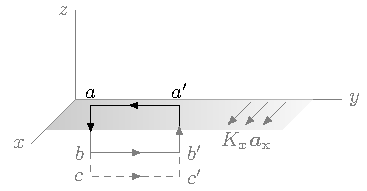
\includegraphics{figMagneticInfiniteSheetMagneticField}
\caption{لامحدود جسامت کے موصل سطح پر سطحی کثافت برقی رو۔}
\label{شکل_مقناطیسی_لامحدود_سطحی_برقی_رو}
\end{subfigure}%
%
\begin{subfigure}{0.5\textwidth}
\centering
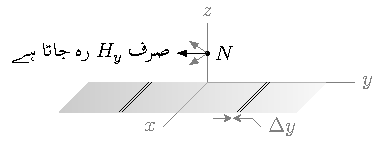
\includegraphics{figMagneticInfiniteSheetDividedIntoWires}
\caption{کسی بھی نقطے کے دونوں جانب فرضی تاروں کے \عددیء{H_z} اجزاء آپس میں ختم ہو جاتے ہیں جبکہ ان کے \عددیء{H_y} اجزاء جمع ہوتے ہیں۔}
\label{شکل_مقناطیسی_دونوں_جانب_زیڈ_اجزاء_ختم}
\end{subfigure}%
\caption{لامحدود سطحی کثافت برقی رو۔}
\label{شکل_مقناطیسی_لامحدود_سطحی_کثافت_برقی_رو}
\end{figure}
شکل \حوالہ{شکل_مقناطیسی_لامحدود_سطحی_کثافت_برقی_رو}-الف میں موصل سطح کے کچھ حصے کو گھیرتی مستطیلی راہ \عددیء{a'abb'} دکھائی گئی ہے جس کے اطراف \عددیء{y_1} اور \عددیء{2z_1} لمبائی رکھتے ہیں۔اس راہ کے \عددیء{z_1} حصوں پر مقناطیسی شدت صفر کے برابر ہے لہٰذا اس حصے پر مقناطیسی شدت کا تکمل بھی صفر کے برابر ہو گا۔راہ کے \عددیء{y_1} اطراف سطح سے دونوں جانب \عددیء{z_1} فاصلے پر ہیں۔سطح کے دونوں اطراف بالکل یکساں مشابہت رکھتے ہیں۔بایوٹ-سیوارٹ کے قانون سے آپ دیکھ سکتے ہیں کہ سطحی کثافت برقی رو  موصل سطح کے اوپر جانب \عددیء{-H_{ya}\ay} جبکہ اس کے نچلی جانب  \عددیء{+H_{yb}\ay} مقناطیسی شدت پیدا کرتا ہے۔مستطیلی راہ \عددیء{Ky_1} برقی رو کو گھیرتی ہے لہٰذا ایمپیئر کے دوری قانون کے تحت
\begin{align*}
H_{ya} y_1+H_{yb} y_1=K_x y_1
\end{align*} 
یا
\begin{align}\label{مساوات_مقناطیسی_لامحدود_دونوں_اطراف}
H_{ya} +H_{yb}=K_x
\end{align} 
ہو گا۔اب اگر موصل سطح کے ایک جانب مستطیلی راہ کا \عددیء{y_1} حصہ قدر دور کرتے ہوئے \عددیء{z_2} فاصلے پر کر دیا جائے تب مندرجہ بالا مساوات 
\begin{align*}
H_{ya} +H_{yc}=K_x
\end{align*} 
صورت اختیار کر لے گی جس سے صاف ظاہر ہے کہ \عددیء{H_{yb}} اور \عددیء{H_{yc}} عین برابر ہیں یعنی مقناطیسی شدت کا دارومدار سطح سے فاصلے پر ہرگز نہیں ہے۔اس طرح تمام ایسے نقطے جو مثبت \عددیء{z} پر پائے جاتے ہوں کا مقناطیسی شدت ایک برابر ہو گا۔یہی کچھ تمام ایسے نقطوں کے لئے بھی درست ہے جو منفی \عددیء{z} پر پائے جاتے ہوں۔ 

سطح کے دونوں اطراف بالکل یکساں مشابہت رکھتے ہیں لہٰذا دونوں جانب  مقناطیسی شدت بھی برابر ہو گا یعنی \عددیء{\abs{\kvec{H}_{ya}}=\abs{\kvec{H}_{yb}}} ہو گا۔اس طرح مساوات \حوالہ{مساوات_مقناطیسی_لامحدود_دونوں_اطراف} سے \عددیء{H_{ya}=H_{yb}=H_y=\tfrac{K_x}{2}} لکھتے ہوئے
\begin{align*}
\kvec{H}_{y}&=-\frac{1}{2}K_x \ax \quad \quad (z>0)\\
\kvec{H}_{y}&=+\frac{1}{2}K_x \ax \quad \quad (z<0)
\end{align*}
حاصل ہوتا ہے جسے  بہتر طور پر 
\begin{align}
\kvec{H}=\frac{1}{2} \kvec{K} \times \aN
\end{align}
لکھا جا سکتا ہے جہاں \عددیء{\aN} موصل سطح کی عمودی اکائی سمتیہ ہے۔

اگر \عددیء{z=-h} پر دوسری لامحدود موصل سطح رکھی جائے جس میں سطحی کثافت برقی رو \عددیء{-K_x\ax} ہو تب دونوں سطحی کثافت برقی رو کا مجموعی مقناطیسی شدت
\begin{gather}
\begin{aligned}
\kvec{H}&=\kvec{K} \times \aN \quad \quad (-h <z < 0)\\
\kvec{H}&=0 \quad \quad \quad \quad  (z<-h, \quad z>0) 
\end{aligned}
\end{gather}
ہو گا۔

ایمپیئر کے دوری قانون کے استعمال میں سب سے مشکل کام ایسی راہ تلاش کرنا ہے جس پر مقناطیسی میدان یا راہ کے عمودی ہو اور یا پھر اس کی قیمت مستقل ہو۔جہاں قبل از وقت ایسا جاننا ممکن نہ ہو وہاں بایوٹ-سیوارٹ کا قانون ہی قابل استعمال ہو گا۔ 

\حصہ{گردش}
آپ کو یاد ہو گا کہ ہم نے گاؤس کے قانون کو انتہائی چھوٹی حجم پر لاگو کرتے ہوئے  \اصطلاح{پھیلاو} کی مساوات حاصل کی تھی۔اس حصے میں ہم ایمپیئر کے دوری قانون کو انتہائی چھوٹی بند راہ پر استعمال کرتے ہوئے \اصطلاح{گردش}\فرہنگ{گردش}\حاشیہب{curl}\فرہنگ{curl} کی مساوات حاصل کریں گے۔
\begin{figure}
\centering
\includegraphics{figGaussCurlDefined}
\caption{گردش کی تعریف۔ }
\label{شکل-مقناطیسی_گردش_تعریف}
\end{figure}

کارتیسی محدد میں ہم کسی نقطے \عددیء{N} پر  \عددیء{\Delta x} اور \عددیء{\Delta y} اطراف کی چھوٹی بند راہ لیتے ہیں۔شکل \حوالہ{شکل-مقناطیسی_گردش_تعریف} میں اس چھوٹی بند راہ کو دکھایا گیا ہے جو رقبہ \عددیء{\Delta x \Delta y} کو گھیرتی ہے۔اس رقبے کے عین وسط میں نقطہ \عددیء{(x_0,y_0,z_0)} پر مقناطیسی شدت 
\begin{align*}
\kvec{H}_0&=H_x(x_0,y_0,z_0)\ax+H_y(x_0,y_0,z_0)\ay+H_z(x_0,y_0,z_0)\az\\
&=H_{x0}\ax+H_{y0}\ay+H_{z0}\az
\end{align*}
کے برابر ہے۔ایمپیئر کے دوری قانون کے تحت اس بند راہ کے گرد مقناطیسی شدت کا تکمل رقبہ \عددیء{\Delta x \Delta y} سے گزرتی برقی رو کے برابر ہو گا۔آئیں اس تکمل کو حاصل کریں۔ایسا کرنے کی خاطر ہم بند راہ پر\عددیء{1} سے \عددیء{2} کی طرف چلتے ہوئے پورا چکر کاٹیں گے۔یوں راہ کے پہلے حصے \عددیء{1} تا \عددیء{2} پر تکمل تقریباً 
\begin{align}\label{مساوات_مقناطیسی_پہلے_حصہ_تکمل}
\left( \kvec{H} \cdot \dif \kvec{L}\right)_{12}=H_{y12} \Delta y 
\end{align}
کے برابر ہو گا جہاں \عددیء{\Delta y} لمبائی پر مقناطیسی شدت کے قیمت میں تبدیلی کو رد کرتے ہوئے اسے  پوری لمبائی پر \عددیء{H_{y12}} کے برابر لیا گیا۔ہمیں رقبے کے عین وسط میں مقناطیسی شدت معلوم ہے البتہ راہ کے پہلے حصے پر ہمیں اس کے بارے میں معلومات فراہم نہیں ہے۔ایسی صورت میں ہمیں \اصطلاح{ٹیلر تسلسل}\فرہنگ{ٹیلر تسلسل}\حاشیہب{Taylor series}\فرہنگ{Taylor series} بروئے کار لانا ہو گا۔

ٹیلر تسلسل
\begin{align*}
f(x+\delta x)=f(x)+\frac{1}{1!}\frac{\partial f}{\partial x} \delta x + \frac{1}{2!}\frac{\partial^2 f}{\partial x^2} (\delta x)^2+\cdots
\end{align*}
سے آپ بخوبی واقف ہیں جہاں \عددیء{\tfrac{\partial f}{\partial x}} اور دیگر تفرق نقطہ \عددیء{x} پر حاصل کئے جاتے ہیں۔اگر اس میں \عددیء{\delta x =\tfrac{\Delta x}{2}} پر کیا جائے تو اس کی نئی شکل
\begin{align*}
f(x+\frac{\Delta x}{2})=f(x)+\frac{1}{1!}\frac{\partial f}{\partial x} \frac{\Delta x}{2} + \frac{1}{2!}\frac{\partial^2 f}{\partial x^2} \left(\frac{\Delta x}{2}\right)^2+\cdots
\end{align*}
حاصل ہوتی ہے جسے ہم اب استعمال کرتے ہیں۔


اگر نقطہ \عددیء{(x_0,y_0,z_0)} پر تفاعل \عددیء{H_y} کی قیمت \عددیء{H_y(x_0,y_0,z_0)} ہو تب نقطہ \عددیء{(x_0+\tfrac{\Delta x}{2},y_0,z_0)} پر اس کی قیمت مسئلہ ٹیلر سے 
\begin{align*}
H_y(x_0+\tfrac{\Delta x}{2},y_0,z_0)&=H_y(x_0,y_0,z_0)+\frac{\partial H_y}{\partial x} \frac{\Delta x}{2}+\cdots\\
&=H_{y0}+\frac{\partial H_y}{\partial x} \frac{\Delta x}{2}+\cdots
\end{align*}
حاصل ہوتی ہے جہاں \عددیء{\tfrac{\partial H_y}{\partial x}} کو نقطہ \عددیء{(x_0,y_0,z_0)} پر حاصل کیا جاتا ہے۔راہ \عددیء{1} تا \عددیء{2} پر مقناطیسی شدت کی قیمت ٹیلر تسلسل کے پہلے دو اجزاء سے حاصل کرتے ہوئے
\begin{align}\label{مساوات_مقناطیسی_راہ_پہلے_حصے_پر_شدت}
H_{y12} \overset{.}{=}H_{y0}+\frac{\partial H_y}{\partial x} \frac{\Delta x}{2}
\end{align}
مساوات \حوالہ{مساوات_مقناطیسی_پہلے_حصہ_تکمل} کو
\begin{align}\label{مساوات_مقناطیسی_پہلے_حصہ_تکمل_الف}
\left( \kvec{H} \cdot \dif \kvec{L}\right)_{12}\overset{.}{=}\left(H_{y0}+\frac{\partial H_y}{\partial x} \frac{\Delta x}{2} \right)\Delta y 
\end{align}
لکھا جا سکتا ہے۔

مساوات \حوالہ{مساوات_مقناطیسی_راہ_پہلے_حصے_پر_شدت} کو یوں بھی حاصل کیا جا سکتا ہے۔چھوٹے رقبے کے وسط میں \عددیء{x} کے ساتھ \عددیء{H_y} تبدیل ہونے کی شرح \عددیء{\tfrac{\partial H_y}{\partial x}} ہے۔ یوں اگر \عددیء{x} میں \عددیء{\Delta x} تبدیلی پیدا ہو تب  \عددیء{H_y} میں تبدیلی تقریباً 
 \عددیء{\tfrac{\partial H_y}{\partial x}\Delta x} ہو گی اور یوں اس کی نئی قیمت تقریباً \عددیء{H_y+\tfrac{\partial H_y}{\partial x}\Delta x} ہو گی۔اسی طرح اگر \عددیء{x} میں \عددیء{\tfrac{\Delta x}{2}} تبدیلی پیدا ہو تب  \عددیء{H_y} میں تبدیلی تقریباً \عددیء{\tfrac{\partial H_y}{\partial x}\tfrac{\Delta x}{2}} ہو گی اور یوں اس کی نئی قیمت تقریباً \عددیء{H_y+\tfrac{\partial H_y}{\partial x}\tfrac{\Delta x}{2}} ہو گی۔اب رقبے کے وسط سے  \عددیء{+\tfrac{\Delta x}{2}} فاصلے پر  \عددیء{1} تا \عددیء{2} راہ کا درمیانہ نقطہ ہے لہٰذا یہاں
\begin{align}\label{مساوات_مقناطیسی_راہ_پہلے_حصے_پر_شدت_دوبارہ}
H_{y12}\overset{.}{=}H_{y0}+\frac{\partial H_y}{\partial x}\frac{\Delta x}{2}
\end{align}
ہو گا جو عین مساوات \حوالہ{مساوات_مقناطیسی_راہ_پہلے_حصے_پر_شدت} ہی  ہے۔

راہ کے اگلے حصے یعنی \عددیء{2} تا \عددیء{3} یہی کچھ کرتے ہوئے
\begin{align}\label{مساوات_مقناطیسی_پہلے_حصہ_تکمل_ب}
\left( \kvec{H} \cdot \dif \kvec{L}\right)_{23}=H_{x23}(-\Delta x) \overset{.}{=}-\left(H_{x0}+\frac{\partial H_x}{\partial y} \frac{\Delta y}{2} \right)\Delta x 
\end{align}
جبکہ \عددیء{3} تا \عددیء{4} پر
\begin{align}\label{مساوات_مقناطیسی_پہلے_حصہ_تکمل_پ}
\left( \kvec{H} \cdot \dif \kvec{L}\right)_{34}=H_{34}(-\Delta y)\overset{.}{=}-\left(H_{y0}-\frac{\partial H_y}{\partial x} \frac{\Delta x}{2} \right)\Delta y 
\end{align}
اور \عددیء{4} تا \عددیء{1} پر
\begin{align}\label{مساوات_مقناطیسی_پہلے_حصہ_تکمل_ت}
\left( \kvec{H} \cdot \dif \kvec{L}\right)_{41}=H_{x41}\Delta x \overset{.}{=}\left(H_{x0}-\frac{\partial H_x}{\partial y} \frac{\Delta y}{2} \right)\Delta x 
\end{align}
حاصل ہوتے ہیں۔مساوات  \حوالہ{مساوات_مقناطیسی_پہلے_حصہ_تکمل_الف}، مساوات \حوالہ{مساوات_مقناطیسی_پہلے_حصہ_تکمل_ب}، مساوات \حوالہ{مساوات_مقناطیسی_پہلے_حصہ_تکمل_پ} اور مساوات \حوالہ{مساوات_مقناطیسی_پہلے_حصہ_تکمل_ت} کو جمع کرتے ہوئے پورے بند راستے کا تکمل
\begin{align}
\oint \kvec{H} \cdot \dif \kvec{L}\overset{.}{=}\left(\frac{\partial H_y}{\partial x}-\frac{\partial H_x}{\partial y} \right)\Delta x \Delta y
\end{align}
حاصل ہوتا ہے۔اگر اس چھوٹے بند راہ کے گھیرے رقبے پر کثافت برقی رو
\begin{align*}
\kvec{J}=J_x \ax+J_y\ay+J_z \az
\end{align*}
ہو تب اس رقبے سے \عددیء{J_z \Delta x \Delta y} برقی رو گزرے گی۔ ایمپیئر کے دوری قانون کے تحت بند راہ کا تکمل اور رقبے سے گزرتی برقی رو برابر ہوں گے یعنی
\begin{align*}
\oint \kvec{H} \cdot \dif \kvec{L}\overset{.}{=}\left(\frac{\partial H_y}{\partial x}-\frac{\partial H_x}{\partial y} \right)\Delta x \Delta y\overset{.}{=}J_z \Delta x \Delta y
\end{align*}
ہو گا جسے
\begin{align*}
\frac{\oint \kvec{H} \cdot \dif \kvec{L}}{\Delta x \Delta y}\overset{.}{=}\frac{\partial H_y}{\partial x}-\frac{\partial H_x}{\partial y}\overset{.}{=}J_z
\end{align*}
لکھا جا سکتا ہے۔رقبے کو جتنا چھوٹا کیا جائے مندرجہ بالا مساوات اتنا ہی زیادہ درست ہو گا حتیٰ کہ \عددیء{\Delta x \to 0} اور \عددیء{\Delta y \to 0} کی صورت میں یہ مکمل طور پر درست ہو گا اور یوں مساوات میں تقریباً برابر کی علامت \عددیء{\overset{.}{=}} کی جگہ بالکل برابر \عددیء{=} کی علامت استعمال کی جائے گی یعنی
\begin{align}\label{مساوات_مقناطیسی_گردش_الف}
\lim_{\overset{\Delta x \to 0}{\Delta y \to 0}}\frac{\oint \kvec{H} \cdot \dif \kvec{L}}{\Delta x \Delta y}=\frac{\partial H_y}{\partial x}-\frac{\partial H_x}{\partial y}=J_z
\end{align}
لکھا جائے گا۔

اگر ہم کارتیسی محدد کے بقایا دو محدد کے عمودی چھوٹے رقبے لیں اور مندرجہ بالا عمل دہرائیں تو ہمیں
\begin{align}\label{مساوات_مقناطیسی_گردش_ب}
\lim_{\overset{\Delta y \to 0}{\Delta z \to 0}}\frac{\oint \kvec{H} \cdot \dif \kvec{L}}{\Delta y \Delta z}=\frac{\partial H_z}{\partial y}-\frac{\partial H_y}{\partial z}=J_x
\end{align}
اور
\begin{align}\label{مساوات_مقناطیسی_گردش_پ}
\lim_{\overset{\Delta z \to 0}{\Delta x \to 0}}\frac{\oint \kvec{H} \cdot \dif \kvec{L}}{\Delta z \Delta x}=\frac{\partial H_x}{\partial z}-\frac{\partial H_z}{\partial x}=J_y
\end{align}
حاصل ہوں گے۔ مساوات \حوالہ{مساوات_مقناطیسی_گردش_ب} میں چھوٹے رقبے کے اطراف \عددیء{\Delta y} اور \عددیء{\Delta z} ہیں جس سے \عددیء{J_x \Delta y \Delta z} برقی رو گزرتی ہے۔اسی طرح مساوات \حوالہ{مساوات_مقناطیسی_گردش_پ} میں چھوٹے رقبے کے اطراف \عددیء{\Delta z} اور \عددیء{\Delta x} ہیں جس سے \عددیء{J_y \Delta z \Delta x} برقی رو گزرتی ہے۔

ایمپیئر کے دوری قانون سے شروع کرتے ہوئے ہم نے مساوات \حوالہ{مساوات_مقناطیسی_گردش_الف}، مساوات \حوالہ{مساوات_مقناطیسی_گردش_ب} اور مساوات \حوالہ{مساوات_مقناطیسی_گردش_پ} حاصل کئے جو مقناطیسی شدت کے بند تکمل فی اکائی رقبہ کو گھیرے گئے کثافت برقی رو کے برابر ٹہراتے ہیں۔کسی بھی متغیرہ کے بند تکمل فی اکائی رقبہ کو اس متغیرہ کی \اصطلاح{گردش}\فرہنگ{گردش}\حاشیہب{curl}\فرہنگ{curl} کہتے ہیں۔انتہائی چھوٹے رقبے کے گرد گردش کرتے ہوئے کسی بھی متغیرہ کے بند تکمل کو اس نقطے پر متغیرہ کے گھومنے یا  گردش کی ناپ تصور کی جا سکتی ہے۔اسی لئے اس عمل کو \اصطلاح{گردش} کہا جاتا ہے۔

کسی بھی سمتیہ کا گردش بھی سمتیہ ہو گا۔گردش کا کوئی بھی جزو انتہائی چھوٹے سیدھے رقبے کے گرد سمتیہ کے بند تکمل فی یہی رقبہ کے برابر ہو گا جہاں بند تکمل کی راہ درکار جزو کے عمودی سطح میں پایا جاتا ہو اور رقبے کی قیمت صفر کے قریب سے قریب تر ہو۔گردش کی یہ تعریف کسی بھی محدد پر مبنی نہیں ہے۔اس تعریف کی حسابی شکل
\begin{align*}
\kvec{H} \textrm{گردش}=\lim_{\Delta S_n \to 0} \frac{\oint \kvec{H} \cdot \dif \kvec{L}}{\Delta S_n}
\end{align*}
ہے جہاں \عددیء{\kvec{H}} کی گردش حاصل کی گئی ہے۔اس مساوات میں \عددیء{\Delta S_n} وہ چھوٹا سیدھا رقبہ ہے جس کے گرد \عددیء{\kvec{H}} کا بند تکمل حاصل کیا گیا ہے۔گردش از خود سیدھے  سطح کے عمودی ہو گا۔ رقبہ \عددیء{\Delta S_n} لکھتے ہوئے زیر نوشت میں \عددیء{n} اسی حقیقت کی یاد دہانی کراتا ہے کہ رقبے اور گردش کے درمیان نوے درجے کا زاویہ پایا جاتا ہے۔

کارتیسی محدد میں گردش \عددیء{\kvec{H}}  کے \عددیء{x}، \عددیء{y} اور \عددیء{z} اجزاء مساوات \حوالہ{مساوات_مقناطیسی_گردش_ب}، مساوات \حوالہ{مساوات_مقناطیسی_گردش_پ} اور مساوات \حوالہ{مساوات_مقناطیسی_گردش_الف} بالترتیب دیتے ہیں لہٰذا
\begin{align}
\kvec{H} \textrm{گردش}=\left(\frac{\partial H_z}{\partial y}-\frac{\partial H_y}{\partial z} \right)\ax+\left( \frac{\partial H_x}{\partial z}-\frac{\partial H_z}{\partial x}\right)\ay+\left(\frac{\partial H_y}{\partial x}-\frac{\partial H_x}{\partial y} \right)\az
\end{align}
لکھا جا سکتا ہے۔اس مساوات کو قالب کے  \اصطلاح{حتمی قیمت}\فرہنگ{قالب!حتمی قیمت}\حاشیہب{determinant}\فرہنگ{determinant} کی شکل میں
\begin{align}
\kvec{H} \textrm{گردش}=
\begin{vmatrix}
\ax & \ay & \az\\
\frac{\partial }{\partial x}&\frac{\partial }{\partial y}&\frac{\partial }{\partial z}\\
H_x & H_y & H_z
\end{vmatrix}
\end{align}
لکھا جا سکتا ہے۔صفحہ \حوالہصفحہ{مساوات-گاؤس_نیبلا} پر مساوات \حوالہ{مساوات-گاؤس_نیبلا} نیبلا \عددیء{\nabla} کے عمل کو بیان کرتا ہے جسے یہاں دوبارہ پیش کرتے ہیں
\begin{align*}
\nabla= \frac{\partial}{\partial x}\ax+\frac{\partial}{\partial y} \ay+\frac{\partial}{\partial z}\az
\end{align*}

اور صفحہ \حوالہصفحہ{مساوات_سمتیات_سمتی_ضرب_قالب_شکل} پر مساوات \حوالہ{مساوات_سمتیات_سمتی_ضرب_قالب_شکل} دو سمتیات کا سمتی ضرب دیتا ہے۔ان  سے گردش نہایت خوبصورتی سے
\begin{align}
\kvec{H} \textrm{گردش}=\nabla \times \kvec{H}
\end{align}
لکھی جا سکتی ہے۔

%==================
\جزوحصہ{نلکی محدد میں گردش}
نلکی محدد میں \عددیء{J_z} کثافت برقی رو کے عمودی سیدھی سطح پر چھوٹا رقبہ لیتے ہیں۔ایسے رقبے کے اطراف \عددیء{\Delta \rho} اور \عددیء{\rho \Delta \phi} ہوں گے۔اس رقبے کو وسط میں
\begin{align*}
\kvec{H}_0(\rho_0,\phi_0,z_0)&=H_{\rho 0}\arho+H_{\phi 0}\aphi+H_{z 0}\az
\end{align*}
ہو گا۔کارتیسی محدد میں رقبے کے وسط سے \عددیء{+\tfrac{\Delta x}{2}} اور \عددیء{-\tfrac{\Delta x}{2}} فاصلے پر اطراف کی لمبائیاں عین برابر تھیں۔نلکی محدد میں رقبے کے وسط سے \عددیء{+\tfrac{\Delta \rho}{2}} فاصلے پر طرف کی لمبائی \عددیء{(\rho_0+\tfrac{\Delta \rho}{2})\Delta \phi} جبکہ  وسط سے \عددیء{-\tfrac{\Delta \rho}{2}} فاصلے پر طرف کی لمبائی \عددیء{(\rho_0-\tfrac{\Delta \rho}{2})\Delta \phi} ہے۔انہیں اطراف پر مقناطیسی شدت  بالترتیب
\begin{align*}
H_{\phi 12}\overset{.}{=}H_{\phi 0}+\frac{\partial H_\phi}{\partial \rho}\frac{\Delta \rho}{2}
\end{align*}
اور
\begin{align*}
H_{\phi 34}\overset{.}{=}H_{\phi 0}-\frac{\partial H_\phi}{\partial \rho}\frac{\Delta \rho}{2}
\end{align*}
ہو گی جہاں \عددیء{\tfrac{\partial H_\phi}{\partial \rho}} چھوٹے رقبے کے وسط میں حاصل کیا جائے گا۔یوں \عددیء{1} سے \عددیء{2} جانب چھوٹے رقبے کے گرد چکر کاٹتے ہوئے ان دو اطراف پر تکمل
\begin{align*}
(\kvec{H} \cdot \dif \kvec{L})_{12}&\overset{.}{=}\left(H_{\phi 0}+\frac{\partial H_\phi}{\partial \rho}\frac{\Delta \rho}{2} \right)\left(\rho_0 +\frac{\Delta \rho}{2} \right)\Delta \phi\\
&\overset{.}{=}\left[H_{\phi 0} \rho_0+H_{\phi 0} \frac{\Delta \rho}{2}+\rho_0 \frac{\partial H_\phi}{\partial \rho}\frac{\Delta \rho}{2}+\frac{\partial H_\phi}{\partial \rho} \left(\frac{\Delta \rho}{2} \right)^2\right]\Delta \phi
\end{align*}
اور
\begin{align*}
(\kvec{H} \cdot \dif \kvec{L})_{34}&\overset{.}{=}\left(H_{\phi 0}-\frac{\partial H_\phi}{\partial \rho}\frac{\Delta \rho}{2} \right)\left[-\left(\rho_0 -\frac{\Delta \rho}{2} \right)\Delta \phi\right]\\
&\overset{.}{=}\left[-H_{\phi 0} \rho_0+H_{\phi 0} \frac{\Delta \rho}{2}+\rho_0 \frac{\partial H_\phi}{\partial \rho}\frac{\Delta \rho}{2}-\frac{\partial H_\phi}{\partial \rho} \left(\frac{\Delta \rho}{2} \right)^2\right]\Delta \phi
\end{align*}
ہوں گے۔

چھوٹے رقبے کے وسط سے \عددیء{+\tfrac{\Delta \phi}{2}}  یا \عددیء{-\tfrac{\Delta \phi}{2}} پر  اطراف
 \عددیء{\Delta \rho} لمبائی رکھتے ہیں جبکہ ان پر اوسط شدت بالترتیب
\begin{align*}
H_{\phi 23}\overset{.}{=}H_{\rho 0}+\frac{\partial H_\rho}{\partial \phi}\frac{\Delta \phi}{2}
\end{align*}
اور
\begin{align*}
H_{\phi 41}\overset{.}{=}H_{\rho 0}-\frac{\partial H_\rho}{\partial \phi}\frac{\Delta \phi}{2}
\end{align*}
ہیں۔یوں ان اطراف پر تکمل
\begin{align*}
\left(\kvec{H} \cdot \dif \kvec{L}\right)_{23} \overset{.}{=}\left(H_{\rho 0}+\frac{\partial H_\rho}{\partial \phi}\frac{\Delta \phi}{2} \right)\left(-\Delta \rho \right)
\end{align*}
اور
\begin{align*}
\left(\kvec{H} \cdot \dif \kvec{L}\right)_{41} \overset{.}{=}\left(H_{\rho 0}-\frac{\partial H_\rho}{\partial \phi}\frac{\Delta \phi}{2} \right)\Delta \rho
\end{align*}
ہوں گے۔

یوں پورا تکمل ان چار جوابات کا مجموعہ
\begin{align}\label{مساوات_مقناطیسی_نلکی_پہلا_بند_تکمل}
\oint\kvec{H} \cdot \dif \kvec{L}\overset{.}{=}\left(H_{\phi 0} +\rho_0 \frac{\partial H_\phi}{\partial \rho}-\frac{\partial H_\rho}{\partial \phi}\right)\Delta \rho \Delta \phi
\end{align}
ہو گا۔اس چھوٹے رقبے سے \عددیء{J_z \rho_0 \Delta \rho \Delta \phi} برقی رو گزرے گی۔یوں ایمپیئر کے دوری قانون سے
\begin{align*}
\oint \kvec{H} \cdot \dif \kvec{L}\overset{.}{=}\left(H_{\phi 0} +\rho_0 \frac{\partial H_\phi}{\partial \rho}-\frac{\partial H_\rho}{\partial \phi}\right)\Delta \rho \Delta \phi\overset{.}{=}J_z \rho_0 \Delta \rho \Delta \phi
\end{align*}
یعنی
\begin{align*}
\frac{\oint \kvec{H} \cdot \dif \kvec{L}}{\rho_0 \Delta \rho \Delta \phi}\overset{.}{=}\left(\frac{H_{\phi 0}}{\rho_0} +\frac{\partial H_\phi}{\partial \rho}-\frac{1}{\rho_0}\frac{\partial H_\rho}{\partial \phi}\right)\overset{.}{=}J_z
\end{align*}
لکھا جا سکتا ہے۔اگر \عددیء{\Delta \rho} اور \عددیء{\Delta \phi} کو کم سے کم کرتے ہوئے صفر کے قریب تر کر دیا جائے تب مندرجہ بالا مساوات بالکل درست ہو گا اور تقریباً برابر کی علامت \عددیء{\overset{.}{=}} کی جگہ برابر کی علامت \عددیء{=} استعمال کی جائے گی۔اس طرح گردش کا پہلا جزو 
\begin{align}
\lim_{\overset{\Delta \rho \to 0}{\Delta \phi \to 0}}\frac{\oint \kvec{H} \cdot \dif \kvec{L}}{\rho_0 \Delta \rho \Delta \phi}=\left(\frac{H_{\phi 0}}{\rho_0} +\frac{\partial H_\phi}{\partial \rho}-\frac{1}{\rho_0}\frac{\partial H_\rho}{\partial \phi}\right)=J_z
\end{align}
لکھا جا سکتا ہے۔

اس سے پہلے کہ ہم گردش کے بقایا دو اجزاء بھی حاصل کریں، آئیں مساوات \حوالہ{مساوات_مقناطیسی_نلکی_پہلا_بند_تکمل} کو قدر مختلف اور بہتر طریقے سے حاصل کریں۔اگر ہم کسی نقطے  کے 
 \عددیء{-\tfrac{\Delta \phi}{2}} سے نقطے کے \عددیء{+\tfrac{\Delta \phi}{2}} تک حرکت کریں تو ہم \عددیء{\rho \Delta \phi}  فاصلہ طے کریں گے۔اس راہ پر تکمل تقریباً
\begin{align*}
\kvec{H} \cdot \dif \kvec{L}=H_{\phi}\rho \Delta \phi
\end{align*}
 کے برابر ہو گا۔اس تکمل کو تفاعل \عددیء{g} تصور کرتے ہوئے  یعنی \عددیء{g=H_{\phi}\rho \Delta \phi} لیتے ہوئے  ہم دیکھتے ہیں کہ اگر ہم چھوٹے رقبے کے وسط سے رداسی سمت میں  \عددیء{+\tfrac{\Delta \rho}{2}} حرکت کریں تو اس تفاعل کی قیمت میں تبدیلی
\begin{align*}
\Delta (\kvec{H} \cdot \dif \kvec{L})=\frac{\partial g}{\partial \rho}\frac{\Delta \rho}{2}=\frac{\partial (H_{\phi}\rho \Delta \phi)}{\partial \rho} \frac{\Delta \rho}{2}
\end{align*}
لکھی جا سکتی ہے جہاں \عددیء{\tfrac{\partial (H_{\phi}\rho \Delta \phi)}{\partial \rho}} کو چھوٹے رقبے کے وسط پر حاصل کیا جاتا ہے جہاں رداس \عددیء{\rho_0} کے برابر ہے۔چونکہ چھوٹے رقبے کے عین وسط پر اس تکمل کی قیمت \عددیء{H_{\phi 0}\rho_0 \Delta \phi} کے برابر ہے لہٰذا وسط سے \عددیء{\tfrac{\Delta \rho}{2}} فاصلے پر تکمل کی قیمت
\begin{align}\label{مساوات_مقناطیسی_نلکی_ایک_دو}
\kvec{H} \cdot \dif \kvec{L}_{12}=H_{\phi}\rho \Delta \phi+\frac{\partial (H_{\phi}\rho \Delta \phi)}{\partial \rho} \frac{\Delta \rho}{2}
\end{align}
ہو گی۔اسی طرح اگر ہم کسی نقطے کے  \عددیء{+\tfrac{\Delta \phi}{2}} سے نقطے کے  \عددیء{-\tfrac{\Delta \phi}{2}} تک حرکت کریں تو اس راہ پر تکمل
\begin{align*}
\kvec{H} \cdot \dif \kvec{L}=H_{\phi} (-\rho \Delta \phi)
\end{align*}
کے برابر ہو گا۔اگر اس نقطے کو چھوٹے رقبے کا وسط تصور کیا جائے تب وسط سے  \عددیء{-\tfrac{\Delta \rho}{2}} فاصلے پر یہی تکمل
\begin{gather}
\begin{aligned}\label{مساوات_مقناطیسی_نلکی_تین_چار}
\kvec{H} \cdot \dif \kvec{L}_{34}&=-H_{\phi}\rho \Delta \phi-\frac{\partial (H_{\phi}\rho \Delta \phi)}{\partial \rho} \left(-\frac{\Delta \rho}{2}\right)\\
&=-H_{\phi}\rho \Delta \phi+\frac{\partial (H_{\phi}\rho \Delta \phi)}{\partial \rho} \frac{\Delta \rho}{2}
\end{aligned}
\end{gather}
ہو گا۔

اسی طرح کسی بھی نقطے پر \عددیء{-\tfrac{\Delta \rho}{2}} تا \عددیء{+\tfrac{\Delta \rho}{2}} حرکت کرتے ہوئے تکمل کی قیمت \عددیء{H_{\rho} \Delta \rho} ہو گی۔اس نقطے سے \عددیء{-\tfrac{\Delta \phi}{2}} پر تکمل کی قیمت میں تبدیلی رو نما ہو گی جسے
\begin{align*}
\Delta  (\kvec{H} \cdot \dif \kvec{L})=\frac{\partial (H_{\rho} \Delta \rho)}{\partial \phi}\left(-\frac{\Delta \phi}{2}\right)
\end{align*}
لکھا جا سکتا ہے اور یوں تکمل کی نئی قیمت
\begin{align*}
\kvec{H} \cdot \dif \kvec{L}=H_{\rho} \Delta \rho-\frac{\partial (H_{\rho} \Delta \rho)}{\partial \phi}\frac{\Delta \phi}{2}
\end{align*}
ہو گی۔اگر چھوٹے رقبے کے عین وسط کو یہی نقطہ تصور کیا جائے تب مندرجہ بالا مساوات \عددیء{4} تا \عددیء{1} پر تکمل دیتا ہے یعنی
\begin{align}\label{مساوات_مقناطیسی_نلکی_چار_ایک}
\kvec{H} \cdot \dif \kvec{L}_{41}=H_{\rho} \Delta \rho-\frac{\partial (H_{\rho} \Delta \rho)}{\partial \phi}\frac{\Delta \phi}{2}
\end{align}
اسی طرح کسی بھی نقطے پر \عددیء{+\tfrac{\Delta \rho}{2}} تا \عددیء{-\tfrac{\Delta \rho}{2}} حرکت کرتے ہوئے تکمل کی قیمت
\begin{align*}
\kvec{H} \cdot \dif \kvec{L}=H_{\rho}(-\Delta \rho)
\end{align*}
ہو گی۔اس نقطے کو چھوٹے رقبے کا وسط تصور کرتے ہوئے وسط  سے \عددیء{+\tfrac{\Delta \phi}{2}} پر یہی تکمل
\begin{align}\label{مساوات_مقناطیسی_نلکی_دو_تین}
\kvec{H} \cdot \dif \kvec{L}_{23}=-H_{\rho} \Delta \rho-\frac{\partial (H_{\rho} \Delta \rho)}{\partial \phi}\frac{\Delta \phi}{2}
\end{align}
کے برابر ہو گا۔

مساوات \حوالہ{مساوات_مقناطیسی_نلکی_ایک_دو}، مساوات \حوالہ{مساوات_مقناطیسی_نلکی_تین_چار}، مساوات \حوالہ{مساوات_مقناطیسی_نلکی_چار_ایک} اور مساوات \حوالہ{مساوات_مقناطیسی_نلکی_دو_تین} کا مجموعہ چھوٹے رقبے کے گرد پورا تکمل دیتا ہے یعنی
\begin{gather}
\begin{aligned}\label{مساوات_مقناطیسی_نلکی_پہلا_بند_تکمل_دوبارہ}
\oint \kvec{H} \cdot \dif \kvec{L}&=\frac{\partial (H_{\phi}\rho \Delta \phi)}{\partial \rho}\Delta \rho-\frac{\partial (H_{\rho} \Delta \rho)}{\partial \phi}\Delta \phi\\
&=\left[\frac{\partial (H_{\phi}\rho )}{\partial \rho}-\frac{\partial H_{\rho}}{\partial \phi}\right] \Delta \rho\Delta \phi
\end{aligned}
\end{gather}
جہاں تفرق رقبے کے وسط پر حاصل کئے جاتے ہیں۔اس مساوات کو یوں بھی لکھا جا سکتا ہے
\begin{align*}
\oint \kvec{H} \cdot \dif \kvec{L}&=\left[H_{\phi 0} +\rho_0 \frac{\partial H_{\phi}}{\partial \rho}-\frac{\partial H_{\rho}}{\partial \phi}\right] \Delta \rho\Delta \phi
\end{align*}
جو بالکل مساوات \حوالہ{مساوات_مقناطیسی_نلکی_پہلا_بند_تکمل} ہی ہے۔یاد رہے کہ \عددیء{\tfrac{\partial (H_{\phi}\rho)}{\partial \rho}} کو اجزاء کی صورت میں لکھتے ہوئے رقبے کے وسط کی قیمتیں پر کی جاتی ہیں۔یوں رداس \عددیء{\rho_0}  اور مقناطیسی شدت \عددیء{H_{\phi 0}} کے برابر ہوں گے۔

آئیں اب نلکی محدد میں گردش کے بقایا دو اجزاء بھی حاصل کریں۔
%===================
